\subsectionlink{その他の実験領域}
前の各節では、中間的尺度および巨視的尺度で異なる状態の重ね合わせを生成・検出し、その漸進的デコヒーレンスを観測できた実験を述べた。これらでは、実験室で観測された量子から古典への現象を、デコヒーレンスが定性的・定量的に説明した。

同じように、ただし別の視点から、ある実験で重ね合わせ状態を生成・観測できない原因を理解するうえでも、デコヒーレンスは役立つ。本節では、現在までに得られたものよりも、さらに大きい非古典的重ね合わせを、将来生成・観測するための有望な候補となる、二つの実験領域を述べる。見るように、それらで重ね合わせの生成・観測がこれほど難しい理由を、デコヒーレンスによって定性的・定量的に記述できる。また、実験手順の改善方法を示唆し、実験室で望ましい重ね合わせを作る目標に、さらに近づくことも可能にする。

\subsubsectionlink{Bose--Einstein凝縮体におけるデコヒーレンス}
Bose--Einstein凝縮は、巨視的数の原子が、ある実験では最大$O(10^7)$個まで、量子相転移を起こし、すべての原子が個別性を失って同一量子状態を占める凝縮体となる、量子力学的現象である。したがって凝縮体は、位相を持つ単一の量子力学的$N$粒子波動関数で完全に記述できる。この位相は実験で調べられる。たとえば二つの凝縮体を重ねると、両者の位相差による干渉模様が観測される\cite{ref294,ref296,ref297,ref298,ref299}（図6.25）。最近は、単一凝縮体をコヒーレントに分割し、その後再結合して干渉縞を観測する干渉計も作れるようになった\cite{ref295}（同じく図6.25参照）。

このような量子的性質の実証の成功にもかかわらず、粒子数が巨視的に区別される状態の重ね合わせに、凝縮体を準備する実験は、いくつかの有望な理論提案\cite{ref300,ref301,ref302,ref303,ref304,ref305,ref306}があるにもかかわらず、これまで失敗している。
% 原文 p.283
\hypertarget{srcpage:283}{}\label{srcpage:283}
しかし、関係するデコヒーレンス機構を考慮すれば、この失敗は定性的にも定量的にもよく理解できる。凝縮体の重ね合わせ状態では、デコヒーレンスは主に、凝縮原子と非凝縮原子の間の、弾性・非弾性散乱によることが分かる。
\begin{figure}[htbp]\centering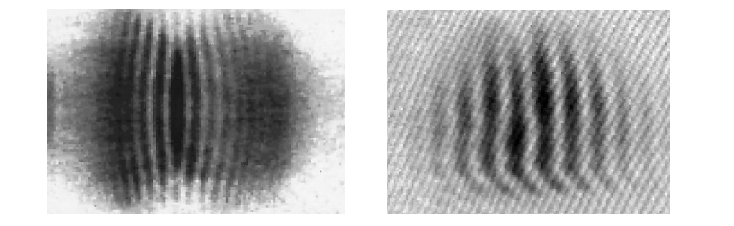
\includegraphics[width=.94\linewidth]{figures/ch06_fig25.pdf}
\caption{Bose--Einstein凝縮体の原子気体密度の干渉模様。左：独立な二凝縮体を重ねたときの、位相差による模様。許可を得て\cite{ref294}から転載。Copyright 1997 by AAAS. 右：凝縮体の「二重スリット」干渉計で得られた干渉縞。単一凝縮体をコヒーレントに分割し、通常の二重スリットの役割を模擬した後、再結合した。許可を得て\cite{ref295}から転載。Copyright 2004 by the American Physical Society.}
\end{figure}

この散乱過程の詳細な模型が作られ（たとえば\cite{ref102}参照）、凝縮体の大きさなどの主要実験パラメーターの関数として、デコヒーレンス時間尺度の現実的予測が得られる。また、これらの模型の知見は、巧妙な実験設計によってデコヒーレンスを最小にする具体的提案を生んだ。改善案には、デコヒーレンスを誘起する非凝縮原子の熱的雲を、より速く蒸発させる、修正した凝縮体トラップ\cite{ref102}、粒子数差状態ではなく相対位相状態の巨視的重ね合わせを作り、環境の選ぶ指針基底を考慮してデコヒーレンスを最小にすること\cite{ref303}、熱的雲の実効的大きさを減らす能動的な環境設計（7.5.3節）\cite{ref102}、重ね合わせ状態のより速い生成\cite{ref306}などがある。各提案は、特定の実験配置に関係する、さまざまなデコヒーレンス機構の分析から導かれる。配置が与えられると、模型は量子・古典境界の位置と、望ましい猫状態を実現するため、その境界を押し進めるには何ができ、何をすべきかを教える。

% 原文 p.284
\hypertarget{srcpage:284}{}\label{srcpage:284}
\subsubsectionlink{量子電気機械系におけるデコヒーレンス}
量子電気機械系、略してQEMSは、さらに大きい非古典的重ね合わせを生成する可能性を持つ、多彩な実験の仲間に、比較的最近加わったものである\cite{ref307}（入門は\cite{ref308,ref309}も参照）。QEMSには、デコヒーレンスと散逸の「振動子・スピン模型」との関連で、5.4.2節ですでに触れた。何十億もの原子が、空間中のよく区別できる二位置の重ね合わせにある、真に機械的な「Schrödingerの子猫」を示すために、QEMSは非常に有望である。この分野の急速な実験進展から、今後数年で、量子から古典への移行の探索で中心的な役割を果たす可能性が高い。

QEMSは、近年のナノテクノロジーの革命の成果である。主要部分は、シリコンなどの結晶材料から作る、小型の両端固定梁または片持ち梁で、典型寸法はnmから$\mu\mathrm m$程度である（図6.26）。梁は小さな機械的共振器として働く。短時間適切な駆動力を加えると、振動運動を始める。

寸法が極めて小さいため、機械系であることを考えると、振動周波数は驚くほど高くできる。最近の実験では、マイクロ波領域の1GHzまで達成した\cite{ref311}。また、共振器の散逸は比較的弱くでき、振幅が有意に減少するまでに、数万回自由振動する。運動は電子トランスデューサーで検出し、対応する電気信号へ変換して読み出す。
\begin{figure}[htbp]\centering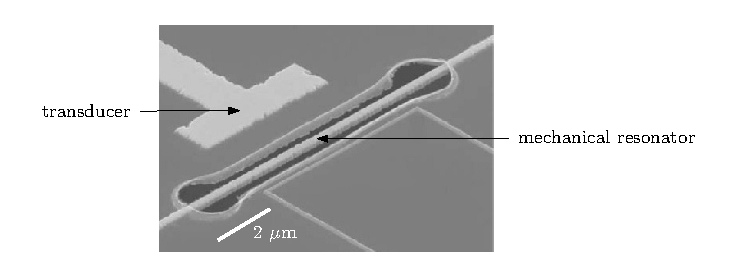
\includegraphics[width=.94\linewidth]{figures/ch06_fig26.pdf}
\caption{Cornell UniversityのKeith Schwabの研究室\cite{ref310}で作られた、量子電気機械系の実験的実現。幅200nm、長さ$8\,\mu\mathrm m$の梁が、固有周波数19.7MHzのナノ機械共振器として働く。電子トランスデューサーで、梁の振動を電気信号へ変換する。許可を得て\cite{ref310}から転載。Copyright 2004 by AAAS.}
\end{figure}
% 原文 p.285
\hypertarget{srcpage:285}{}\label{srcpage:285}
注目すべきことに、共振器の大部分の自由度は、QEMSの典型的動作温度であるmKという低温で「凍結」されるか、トランスデューサーへの結合が無視できる。したがって多くの場合、巨視的共振器は、梁の最低の基本曲げモードに対応する、単一の量子力学的調和振動子として実効的に扱える。QEMSのナノ機械共振器は、何十億もの原子からなり、多数の内部欠陥や不完全さで乱された、巨視的機械物体である。それにもかかわらず、これから述べるように、明確に量子力学的な効果を示せる。

QEMSの主要な特徴は、空間変位への極めて高い感度である。重要な量は、位置検出の量子限界を表す、調和振動子の量子零点変位の不確定性$\Delta x_{\mathrm{zp}}$である。現在実験室で作られるナノ機械共振器では、わずか0.1pm程度である\cite{ref307}。それでも最近の実験では、たとえば図6.26のQEMSを用い、$\Delta x_{\mathrm{zp}}$の数倍に至るまで空間変位を分解できた\cite{ref310}。したがって、量子限界での位置測定という目標に非常に近づいている。

\subsubsectionlink*{QEMSによる機械的「Schrödingerの子猫」の生成法}
研究者たちは、共振器を二つの異なる空間変位のコヒーレント重ね合わせに置き、その漸進的デコヒーレンスを観測する可能性も考えている。特に面白いのは、QEMSが、たとえば超伝導量子ビット（6.3節）やBose--Einstein凝縮体（6.4.1節）よりも、日常世界の物体にはるかに近い、純粋な機械構造であることだ。実現すれば、それは、巨視的で「粗い」通常物質の機械物体が、二つの異なる位置にある重ね合わせを表す。現時点では、そのような重ね合わせはまだ実験室で実現されていないが、具体的提案\cite{ref312}があり、関係するデコヒーレンス・散逸機構の理論研究も進んでいる\cite{ref242,ref313,ref314,ref315}。巨視的距離だけ離れた複数の共振器をもつれさせる考えも、理論的に調べられた\cite{ref316}。量子コンピューターの機械的量子ビットとして使う可能性も、考えられる\cite{ref317}。

Armour、Blencowe、Schwab\cite{ref312}の提案した、QEMSの空間的重ね合わせの生成法を簡単に概説しよう（\cite{ref307}も参照）。基本的考えは、基底状態$|0\rangle$、$|1\rangle$が共振器の異なる二変位へ結合し、しかもそれらの重ね合わせへ比較的容易に準備できる、二状態量子系を使うことである。
% 原文 p.286
\hypertarget{srcpage:286}{}\label{srcpage:286}
\cite{ref312}ではCooper対箱を選んだ（6.3.4節参照）。二基底状態は、超伝導島上の異なる電荷値に対応する。箱と片持ち梁の静電相互作用は、箱が$|0\rangle$か$|1\rangle$かに応じて、共振器に二つの異なる変位を与える（図6.27）。対応する重心位置状態を、$|P_0\rangle$、$|P_1\rangle$と書こう。

箱を$(|0\rangle+|1\rangle)/\sqrt2$の重ね合わせに準備する。\cite{ref312}が示したように、特定の制御パルス列を箱へ加えると、もつれた箱・共振器の重ね合わせ
\begin{equation}|\Psi\rangle=\frac1{\sqrt2}(|0\rangle|P_0\rangle+|1\rangle|P_1\rangle)\tag{6.37}\end{equation}
が得られる。二重心状態の空間的隔たりが十分巨視的なら、Schrödingerの猫型の状態を生成したことになる。共振器が猫の役割を果たし、箱は元の設定の不安定な原子に対応する。

重ね合わせ(6.37)の存在は、Ramsey干渉法（2.2.2節）で確認できる。ある遅延時間後に、Cooper対箱へ追加の制御パルスを加えると、もつれた状態が変換され、
% 原文 p.287
\hypertarget{srcpage:287}{}\label{srcpage:287}
箱を$|0\rangle$または$|1\rangle$に見いだす確率が、遅延時間に振動的に依存する。この依存性は、箱・共振器系が成分状態の古典混合にあるなら現れない。6.3.4節で論じたように、Ramsey法は特徴的なデコヒーレンス時間の情報も与える。
\begin{figure}[htbp]\centering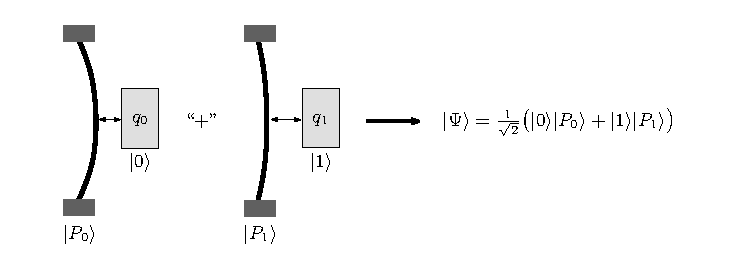
\includegraphics[width=.96\linewidth]{figures/ch06_fig27.pdf}
\caption{Armour、Blencowe、Schwab\cite{ref312}が提案した、ナノ機械共振器の二つの異なる位置の重ね合わせを生成する方法。箱の超伝導島の異なる電荷$q_0$、$q_1$に対応する基底状態$|0\rangle$、$|1\rangle$で記述されるCooper対箱を、共振器へ静電結合する。箱をコヒーレント重ね合わせ$(|0\rangle+|1\rangle)/\sqrt2$に準備し、適切な制御パルス列を加えると、もつれた箱・共振器の重ね合わせ$(|0\rangle|P_0\rangle+|1\rangle|P_1\rangle)/\sqrt2$が得られる。$|P_0\rangle$、$|P_1\rangle$は、共振器の識別できる二つの重心位置に対応する。}
\end{figure}

\subsubsectionlink*{QEMSにおけるデコヒーレンス}
上述の生成法の実用的な実現可能性を評価するには、その重ね合わせに影響するデコヒーレンスの主な源を理解することが重要である。まず、Cooper対箱自体も、もちろんデコヒーレンスを受ける。しかし、6.3.4節で述べたように、$\mu\mathrm s$領域の比較的長い時間は実験的に達成可能である\cite{ref289}。したがって、共振器自体の環境相互作用によるデコヒーレンスに焦点を当てられる。

興味深いことに、現在の実験的証拠\cite{ref318,ref319}、および初期の結果（たとえば\cite{ref320,ref321}）は、QEMSの主な散逸源、したがってデコヒーレンス源も、共振器の最低の基本曲げモードと、共振器内の局在した欠陥との相互作用かもしれないことを示す。これらの欠陥は有効二準位系で、電荷トラップ、不純物原子、弾性中心、共振器表面の結晶構造の乱れによる未結合手など、さまざまな物理的実現を取る。

現時点では、欠陥の基礎にある正確な物理的詳細や、曲げモードとの相互作用は、実験でも理論でも、まだ十分理解されていない。上述の空間的重ね合わせはまだ実現されていないため、QEMSのデコヒーレンスの直接実験データは存在しない。しかし、近年の実験は、散逸の特徴的性質について、貴重な情報を与えた\cite{ref318,ref319}。

散逸には一般にデコヒーレンスが伴うが、その逆は成り立たないので、こうした測定から、デコヒーレンスの性質についても知見を得られる。たとえば散逸データから、欠陥で構成される環境の有効スペクトル密度を取り出せるかもしれない。共振器と欠陥の相互作用の適切な模型があれば、それを使って、関係するデコヒーレンス係数と動力学を計算できる。そして、上述の重ね合わせの特徴的デコヒーレンス率を評価し、生成法の実現可能性を検討できる。ゆえに、QEMSの散逸とデコヒーレンスの現実的模型の開発が、主要な目標の一つとなる\cite{ref242,ref314,ref315}。それは理論的理解を高めるだけでなく、重ね合わせの実験的実現を前進させ、QEMSの実装全般の改善も示唆する。

% 原文 p.288
\hypertarget{srcpage:288}{}\label{srcpage:288}
Armour、Blencowe、Schwabは、最初の提案\cite{ref312}で、5.2節のよく研究された量子Brown運動模型を用い、空間的な箱・共振器重ね合わせ(6.37)のデコヒーレンス時間を評価した。中心調和振動子が基本曲げモードを表し、ほかの調和振動子からなる環境へ弱く結合する。しかし上述のように、mK温度のナノ機械共振器の環境は、欠陥を表す二準位系の集まりとして記述する方が、より現実的かもしれない。これらを量子スピン$1/2$粒子として模型化すれば、振動子・スピン模型が得られる。その弱結合マスター方程式は、5.4.2節で導いた［(5.198)参照］。

しかし、この模型の減衰率の温度依存性［(5.200)参照］は、散逸率が温度とともに増加するというQEMSの実験データ\cite{ref318,ref319}と一致しない。この不一致は、欠陥の少なくとも一部を、さらに別の、デコヒーレンスと散逸を生む環境に強く結合した、スピン$1/2$粒子として扱うべきことを示す（図6.28）。この環境は、スピンのトンネルを非コヒーレントにし、緩和も生じさせ、古典的二準位揺動子に似た欠陥動力学を誘起する。スピン浴から過剰エネルギーを吸収することで、その飽和を防ぐ。したがって、より現実的な模型は、独立なスピン・ボソン模型、すなわち振動子浴と相互作用するスピンを複数個、中心調和振動子へ結合したものかもしれない。この模型の最初の研究は、ごく最近行われた\cite{ref242}。このようにQEMSは、異なるデコヒーレンス・散逸模型を、実験で区別し検証する機会を与える。
\begin{figure}[htbp]\centering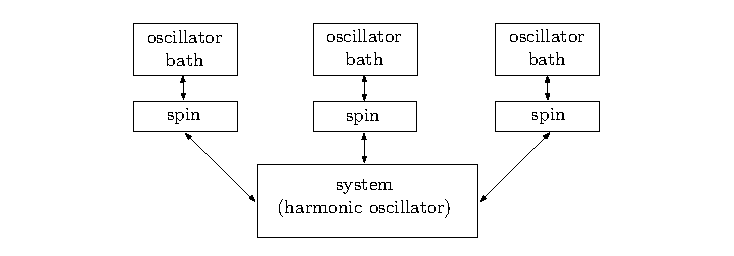
\includegraphics[width=.86\linewidth]{figures/ch06_fig28.pdf}
\caption{QEMSのデコヒーレンスと散逸の、考えられる模型。中心系は、ナノ機械共振器の基本曲げモードを表す調和振動子からなる。これは、スピン$1/2$粒子として模型化した二準位欠陥の集合と相互作用する。さらに各スピンは、散逸的な振動子浴へ結合し、その浴が、そうしなければ容易に飽和するスピン環境から、エネルギーを吸収する。}
\end{figure}

% 原文 p.289
\hypertarget{srcpage:289}{}\label{srcpage:289}
\subsectionlink{展望}
Schrödingerが1935年に猫の逆説を初めて描いたとき、それを純粋な思考実験、経験する巨視的世界へ量子力学を適用したときに生じる、明らかに「不合理な」帰結の例と考えた。しかし、過去数年、比較的小さいとはいえ、それでも巨視的なSchrödingerの猫を、実験室で育て、観測することに、大きな進展があった。本章では、数十個の光子を含む、巨視的に区別できる二状態の重ね合わせの生成（6.1節）、重い$\mathrm C_{70}$分子の干渉模様の観測（6.2節）、逆方向に流れる二つの$\mu\mathrm A$電流の重ね合わせの存在の検証（6.3節）を達成した実験を述べた。

各実験で研究者は、デコヒーレンスの漸進的作用、すなわち環境との相互作用により、重ね合わせがやがて観測できなくなる様子も、明示的に測定できた。こうして、量子から古典への移行の滑らかさを、明瞭に見た。量子状態を古典状態へ不連続に変換するような、固定された障壁は、量子領域と古典領域の間にない。系と環境の相互作用を操作することで、移行の動力学と時間尺度を直接変えられる。

したがって、本章の実験は、デコヒーレンスの範囲が、周囲の巨視的物体の、実効的に瞬時の「局在化」を指すだけよりも、はるかに広いことを示す。デコヒーレンスは、実効的古典性の出現を、漸進的で制御可能な過程として説明する。それは実験室で直接観測・検証でき、標準的量子力学の形式で厳密に理論記述できる。

ここでは、理論と実験の相互作用が非常に密接である。デコヒーレンス時間尺度や、その動力学のほかの性質の測定によって、模型を実験室で直接試せる。そして、模型がどの程度現実的で、物理的に適切かを学ぶ。一方、模型は、既存と将来の実験について貴重な情報を与える。ある配置で、どの段階の「巨視性」で量子から古典への移行を予想すべきか、あるパラメーターの組でどの種の「Schrödingerの子猫」を生成・観測できそうか、さらに「猫らしい」重ね合わせを作るため、実験をどう改善できるかを教える。本章では、理論的方式で提案された特定の重ね合わせの生成を、まだ達成していない二領域、Bose--Einstein凝縮（6.4.1節）と量子電気機械系（6.4.2節）を述べた。それでも、測定データとデコヒーレンス模型を組み合わせれば、望ましい重ね合わせを「見る」のを妨げる、物理的に関係する機構を同定でき、
% 原文 p.290
\hypertarget{srcpage:290}{}\label{srcpage:290}
有害な効果を弱める方法が示唆される。

自然に生じる問いは、巨視的に異なる状態の重ね合わせの実験が、将来どこへ向かうのか、その結果が量子力学の理解や、量子コンピューターなどの大規模量子系の構築に、どのような含意を持つか、ということである。答えは多いので、主要な点を少しだけ挙げよう。

まず、これまで調べた尺度では、既存の実験的証拠は、重ね合わせ原理の根本的限界を示していない。環境との望ましくない相互作用を最小にする適切な設計で、デコヒーレンスを十分制御できる限り、その限界は精密な定量解析が可能だが、「古典的」状態のどのような数の重ね合わせも、生成・観測できるように見える。

したがって、今後数年、巨視的に異なる状態の重ね合わせの、達成可能な「大きさ」の限界を、さらに押し進める多くの実験を見ることになる、といってよい。近いうちに、ウイルスのような、さらに大きい生体分子の干渉模様を観測し、凝縮体やナノ機械共振器の重ね合わせを実現し、超伝導量子ビットのデコヒーレンス時間を飛躍的に延ばせるかもしれない。このような実験は、重ね合わせ原理が破れる可能性を探し続けることによっても動機づけられる。しかし、デコヒーレンスは局所観測者からは見かけの破れを生じさせるので、十分にそれを遮蔽しながら、ユニタリー発展からのずれを誘起する機構には適度に敏感な実験を設計するのは、今後も非常に難しいだろう（8.4節および\cite{ref286,ref322}参照）。

ますます異なる巨視的状態の重ね合わせを生成・観測できることは、その重ね合わせ自体や、デコヒーレンスと量子力学一般に関わる、根本的な解釈上の問いを解かないことを、強調する必要がある。量子状態（2.1節）、特に重ね合わせ状態（2.2.1節）の適切な解釈と物理的意味の問題は、2.2.2節のStern--Gerlach実験のような、微視的設定ですでに明らかである。近年の巨視的重ね合わせ実験は、Schrödingerの猫型の直観に反する色合いを加えるかもしれないが、解釈の根本問題を解きも、深めもしない。

特に、環境を含む全体の量子状態でコヒーレンスが持続することをどう理解するか、したがって、デコヒーレンスの密度行列記述から生じる量子状態の非真正混合を、基礎にある何らかの量子的実在へどう適切に関係づけるかは、基礎論上の論争であり続ける。
% 原文 p.291
\hypertarget{srcpage:291}{}\label{srcpage:291}
ここで論じた型の実験は、少なくとも「実在の本性」についての先入観へ、さらに挑むことで、議論を今後も明るく照らすだろう。純粋にユニタリーな動力学からのずれを、実験が決定的に示す、あるいは排除できるようになれば、量子力学と量子的実在の構造について、新たな知見を得るか、得ざるを得なくなるかもしれない。しかし現在は、本章の驚くべき実験的成果を踏まえても、解釈の問題は残り続ける。
